\chapter{Solution of linear systems}
\label{sec:solution-strategies}

In this \thisref{sec:solution-strategies} we discuss solution strategies for the various linear systems of equations that result from the application of the FEM and BEM techniques discussed in \cref{sec:galerk-meth-llg,sec:hybr-finit-elem}.

We first discuss methods of solving the linear system for the LLG equation assuming the magnetostatic field is known and the magnetostatic field assuming the magnetisation is known.

We then move on to the solution of these combination of these two systems which is non-trivial because of the dense BEM matrix.
The first technique, which is commonly implemented,\footnote{At least \nmag, probably \magpar and \femme use this method.} is to use an ad-hoc \emph{semi}-implicit time integration scheme in which the magnetostatic calculations are handled explicitly.
The second technique, which is novel, is to use a preconditioned Krylov solver in combination with hierarchical matrix techniques in order to efficiently solve the monolithic, \ie fully-implicitly-coupled system.

In the final section we present some numerical experiments comparing the approaches.


\section{Solution of decoupled systems}
\label{sec:llg-only-system}

Efficient solver strategies for Poisson systems (\cref{sec:poisson-jacobian}) such as those involved in the magnetostatics solve are extremely well studied.
One efficent and robust method for solving Poisson systems on unstructured grids is to use the method of conjugate gradients (CG) with algebraic multigrid (AMG) as a preconditioner \cite[Chap. 2]{HowardElmanDavidSilvester2006}.
We implement such a solver using \oomph's preconditioned CG with a relative convergence tolerance of $10^{-8}$.
For preconditioning we use one V(1,1) cycle of \hypre's BoomerAMG preconditioner \cite{hypre} with Gauss-Seidel smoothing, CLJP coarsening and a connection strength threshold of 0.7.


There do not appear to be any efficient, robust and scalable solvers in the literature for the LLG system with linearisation by the Newton-Raphson method.
Typically CVODE's GMRES is used with a generic preconditioner based on approximating the Jacobian as a banded matrix \cite{nmag} \cite{Vasslios}.
This should work for sufficiently small time steps, \ie when the mass matrices of \cref{eq:llg-jacobian} are the dominant term, or when the number of nodes is sufficiently small.
It would not be expected to work efficiently for larger time steps and large numbers of nodes.
Try two solvers in our model but neither are expected to be scalable to large mesh sizes.

The first method used is a direct solve by LU decomposition (using \superlu \cite{superlu} with parameters ??ds).
As discussed in \cref{sec:direct-methods} this method is extremely robust, but also extremely slow for large meshes (??ds what size).

The second method is to use GMRES preconditioned by ILU.
We \oomph's GMRES with left preconditioning, no restarts and a relative convergence tolerance of $10^{-8}$.
For the ILU preconditioner we use \hypre's Euclid with one level of fill in and no drop tolerance.
Incomplete LU decomposition with no fill in was also tested but found to be ineffective, especially for larger time steps.
This method can be efficient for medium sized meshes (up to around 100,000 nodes), but for larger meshes the preconditioner is both slow to assemble and ineffective.
It is also not particularly robust: iteration counts can vary widely depending on problem parameters.

Unfortunately we have not had time to research more effective solvers for the LLG system.


??ds solver for mass matrix in explicit solve?


\section{Solution of the systems from implicit LLG with explicit magnetostatics}
\label{sec:semi-implicit-bem}


When we combine implicit time integration schemes with FEM for the spatial discretisation of the LLG equation, the Newton-Raphson method for linearisation (as discussed in \cref ) and the FEM/BEM for calculation of magnetostatic fields we need to solve a series of systems of linear equations involving the Jacobian matrix.

However, unlike typical FEM computations, these Jacobian matrices are not entirely sparse.
The BEM matrix, $\bm$, derived in \cref{sec:discretisation} appears as a block in the Jacobian.
There are numerous well understood linear solvers, such as those discussed in \cref{sec:solution-lin-sys}, which can be extremely efficient for large sparse systems.
But, at least in their standard form, they are much less efficient for systems involving a dense block. ??ds what do I mean, LU decomposition: massive increase in nnz, multigrid inapplicable, Krylov solvers maybe...

In this section we describe two methods of efficiently dealing with the dense block of the Jacobian.
The first method (which is similar to the methods used in other models) is to replace our implicit time integration scheme with a semi-implicit version.
In this method the magnetostatic calculation is handled explicitly while the rest of the calculation is done implicitly as normal.
This results in decoupled solves for $\phione$, $\phi$ and $\mv$ at each step, and the dense block only appears as a matrix-vector multiply.
However this means that we are no longer using the time integration methods discussed in \cref{sec:some-implicit-time-integrators}, instead we are using some new ad-hoc time integration scheme.
The stability, convergence, geometric integration properties of the original schemes do not necessarily carry over to the semi-implicit versions.
In particular the energy property of IMR does not carry over (see \cref{??}).

An alternative is to construct a linear solver which can efficiently handle the dense block.
We present a novel solver using a preconditioned Krylov method combined with a hierarchical representation of the BEM block.


The alternative to a fully implicit solve is to come up with a semi implicit method.
The idea is to approximate $\phim$ using an explicit time integration method while still using an implicit method for $\mv$.
This means that the system no longer has the properties of the purely implicit method.
We hope that despite this it will retain sufficient stability to allow long time steps.

The strategy is as follows:
\begin{enumerate}
\item Calculate $\phim_0$ from initial condition $\mv_0$.
\item Extrapolate $\phim_n$ to $t_{n+1}$ using a second order formula to get $\hat{\phim}_{n+1}$.
\item Use $\hat{\phim}_{n+1}$ to calculate $\mv_{n+1}$ (implicitly in $\mv_{n+1}$).
\item Calculate $\phione_{n+1}$ using $\mv_{n+1}$.
\item Use boundary values of $\phione_{n+1}$ to get $\phim_{n+1}$.
\item If not finished then goto 2.
\end{enumerate}

A simple second order extrapolation formula (based on Lagrange interpolation \cite[312]{Kincaid2002}) is 
\begin{equation}
  \label{eq:65}
  f(t) = \frac{t - t_1}{t_0 - t_1}f(t_0) + \frac{t - t_0}{t_1 - t_0}f(t_1).
\end{equation}
After substituting in $t=t_{n+1}$, $t_1=t_n$ and $t_0=t_{n-1}$ this gives an expression for the predicted $\phim$ value
\begin{equation}
  \label{eq:66}
  \hat{\phim}_{n+1} = \frac{-\dtx{n+1}}{\dtn} \phim_{n-1} + \frac{\dtx{n+1} + \dtn}{\dtn} \phim_n.
\end{equation}

Note that if we are using the implicit midpoint rule then we actually want to extrapolate $\phim$ to the midpoint, hence we actually use $\dtx{n+1} = \dtx{n+1} /2$ in the above equation.
If we are using the implicit midpoint rule with constant time steps then the extrapolation formula becomes
\begin{equation}
  \label{eq:67}
  \hat{\phim}_{n+1} = \frac{1}{2} \phim_{n-1} + \frac{3}{2} \phim_n,
\end{equation}
which matches with the extrapolation formula given for a different semi-implicit version of the midpoint rule \cite{Serpico2001}.

Notes:
\begin{itemize}
\item stability uncertain: polynomial extrapolation can be dodgy..
\item Need to find error expression for extrapolation
\item talk about relation to FEM (Lagrange polynomials)?
\end{itemize}


Decoupling the system as discussed above means that we only need to solve the LLG system (as discussed in \cref{sec:llg-jacobian}) along with two Poisson systems of size $\sim N$ (as given in \cref{sec:poisson-jacobian}).
Additionally we need to perform a single (dense or hierarchical) matrix multiply of size $N_b$ to calculate the boundary conditions on the $\phim$ Poisson solve.


Since the $\phione$, $\phi$ and $\mv$ systems are decoupled we can use the solvers discussed in \cref{sec:llg-only-system} without any modifications.



\section{Fully implicit}
\label{sec:fully-implicit-bem}

??ds mention TR blows up with semi-implicit + numerical experiments

Solve the entire system as one coupled non-linear pde.
This means that we are using a well understood time integration scheme rather than some relatively unknown approximation.
The downside is that the Jacobian will contain the dense matrix $\bm$, which makes solving the system in a naive manner extremely expensive.
In \thisref{sec:fully-implicit-bem} we will discuss solvers which can make this process comparatively efficient.

Another advantage of this method over the semi-implicit method arises when using IMR.
The energy conservation property of IMR is the most unique of its geometrical integration properties\footnote{A number of explicit integration schemes can obtain length conservation: Cayley transform methods \cite{Lewis2003}, semi-analytical methods \cite{Wiele2010} and various types of semi-implicit midpoint rule methods \cite{Spargo2003} \cite{Mentink2010} (including the one described in \thisref{sec:solution-strategies}).}, but it is lost when a semi-implicit method is used.

To enforce the Dirichlet boundary condition resulting from the collocation method BEM within the Newton solver we use the slightly odd residual
\newcommand{\rphimb}{\rphi_b}
\begin{equation}
  \rphimb(\phim_b, \phione_b) = \bm[\phione_b] - \phim_b.
\end{equation}
Everything else proceeds as normal.

The basic ideas are: avoid calculating an inverse involving the dense block by using an iterative solver, construct a preconditioner such that this iterative solver is efficient, do not use the dense block in the preconditioner.
This means that the dense block only appears as a matrix-vector product (one per iteration), but we can use a hierarchical representation of it to make this almost as efficient as a sparse matrix vector product.


\subsection{Jacobian structure}
\label{sec:bem-jacobian-structure}

As mentioned in \cref{sec:discretisation} the pair of Poisson equations for the FEM/BEM method are essentially the same as those in \cref{sec:galerk-meth-llg}.
The first difference is that there is no coupling from the auxilary potential $\phione$ to the LLG equations, and hence no corresponding $\Pm$ block.
The second difference is that there is an additional coupling between the boundary values of the auxiliary potential and the boundary values of the real potential $\phim$.

With the order of blocks as: $\mv$, $\phim$, $\phione$ the Jacobian is
\begin{equation}
  \Jm = 
  \begin{pmatrix}
    \Fm       & \Pm     &  \\
    \Qm'      & \Am' &  \bm'  \\
    \Qm       &         &   \Am
  \end{pmatrix},
\label{eq:16}
\end{equation}

%% all in one:
% \begin{equation}
%   \Jm = 
%   \begin{pmatrix}
%     \Fm       & \Pm     & \Pm_b  &         &           \\
%     \Qm       & \Am     & \pd{\phim}{\phim_b}  &         &           \\
%     &         & -\Idm  &         &  \bm      \\
%     \Qm       &         &        & \Am     & \pd{\phione}{\phione_b}   \\
%     \Qm_b     &         &        & \pd{\phione_b}{\phione} & \Am_b      
%   \end{pmatrix}
% \end{equation}

where the primed blocks are ones where the boundary and bulk values must be split up because of the BEM boundary condition.
So
\begin{equation}
  \Am' =
  \begin{pmatrix}
    \Am     & \pd{\phim}{\phim_b} \\
    0      & -\Idm  
  \end{pmatrix},
\end{equation}
\begin{equation}
  \Qm' =
  \begin{pmatrix}
    \Qm \\
    0    
  \end{pmatrix},
\end{equation}
and
\begin{equation}
  \bm' =
  \begin{pmatrix}
    0  & 0 \\
    0  & \bm 
  \end{pmatrix}.
\end{equation}


It is worth noting that a slightly different Jacobian struture could be obtained by modifying the derivation in \cref{sec:appl-magn-calc}.
Instead of using $\phim = \phione + \phitwo$ to eliminate $\phitwo$, we use $\hms = - \grad ( \phione + \phitwo)$.
This would result in both of the potentials having a $\Pm$ block, but only one of them having a $\Qm$ block.
It would also reduce the diagonal dominance of $\bm$, which is probably a bad thing ??ds check? are we sure?


\subsection{Solver strategies}
\label{sec:bem-solver-strategies}

The first technique for an efficient strategy is to use a hierarchical matrix representation for $\bm$.
This greatly increases the asymptotic efficiency of operations, for example multiplication only takes $\order{N_b \log N_b}$ instead of $\order{N_b^2}$ time where $N_b$ is the number of boundary nodes.
However this rules out the use of a straightforward direct solver.
Hence we need to use some form of block-wise solver where it is possible to treat seperate blocks differently.
A simple way to do this is to use a Krylov subspace method.
In such a solver all that is needed is a way to calculate matrix-vector products for $J$, which can easily be done in a block-wise manner.

\newcommand{\prcd}{\mathcal{P}}

We test a range of preconditioning approaches:
The first preconditioner is very simple: we do an exact solve (using LU decomposition) of all of $\Jm$ except for the dense block.
That is
\begin{equation}
  \prcd_{1} = 
  \begin{pmatrix}
    \Fm       & \Pm     &  \\
    \Qm'       & \Am'    &   \\
    \Qm       &         &   \Am
  \end{pmatrix}.
\end{equation}
This preconditioner, while much more efficient than an exact solve including the dense block is not very efficient.
However it allows us to test the effect of simply dropping $\Gm'$ from the preconditioner.

The second and third preconditioners are more ambitious, we drop additional blocks in order to make the preconditioner block triangular.
It can then be solved by inverting the diagonal blocks and using back/forward substitution.
So these preconditioners are
\begin{equation}
  \prcd_{2} = 
  \begin{pmatrix}
    \Fm       &           &  \\
    \Qm'       & \Am'&   \\
    \Qm       &           &   \Am
  \end{pmatrix},
  \label{eq:ms-block-prec-drop-p}
\end{equation}
and
\begin{equation}
  \prcd_{3} = 
  \begin{pmatrix}
    \Fm       & \Pm       &  \\
    & \Am' &   \\
    \Qm       &           &   \Am
  \end{pmatrix},
  \label{eq:ms-block-prec-drop-q}
\end{equation}
where $\prcd_{3}$ can obviously be reordered to give a block triangular preconditioner.

Q is a much simpler block (linear, only one term) so probably best to drop that?


However $\prcd_2$ and $\prcd_3$ still require LU decompositions of each of the diagonal blocks in the solution of the preconditioner.
It would be more efficient to approximate their inverses by an iterative process.
Based on the fact that CG preconditioned with AMG is known to be extremely effective for Poisson problems we use an AMG preconditioner for the $\Am$ blocks (recall that CG and GMRES are both Krylov solvers, so the requirements for effective preconditioners are very similar ??ds identical?).
We also try ILU-1 for the $\Fm$ block, but we expect similar restrictions to those discussed in \cref{sec:llg-only-system}.




\section{Numerical experiments}

We now test the performance and robustness of the linear solvers developed in \thisref{sec:solution-strategies}.
The performance and stability of the implicit and semi-implicit time integration schemes will be tested later in \cref{cha:numer-experiments}.


\subsection{Problem definition}

In order to test our solvers we only need to model a single time step of some problem.

Since the vast majority of practical micromagnetics calculations are in three dimensions our test case must be 3D.

The hierarchical matrix library that we are using (\hlib with patches from \nmag) only supports triangular surface elements for co-location BEM, so we need to use a tetrahedral mesh.

There must be sharp corners in order to test the effect of near singular integrals in the FEM/BEM method.

We choose not to use the \mumag standard problem \#4 because both the FEM/BEM method for magnetostatic calculations and the FEM with linear basis functions are exceptionally unsuited for such thin film problems.
FEM/BEM is bad for thin film problems because every single node is on the boundary, hence the dense block is very large.
Standard FEM with linear basis functions is bad because it allows the magnetisation to vary through the thickness of the film, meaning that the problem is 3D instead of 2D!
(It is certainly possible to construct a finite element method which assumes constant magnetisation in one direction, but our purpose here is to test our model not to invent new ones!)

Additionally the magnetisation must vary strongly in space such that there are no accidental symmetries in the test linear system that do not exist in realistic cases.  

Since there are no existing analytical solutions or standard problems which fit our requirements we will choose a simple cuboid.

??ds damping

??ds initial m?

??ds quadratures

??ds applied field

Since the only difference to the linear systems with different time integration methods is slight change on constant in front of mass matrix we run all experiments using IMR.


All experiments are run on a single core of an intel-i7...


\subsection{Results}

First we show the timing results for a direct solve including the dense block. 
For obvious reasons only very small systems are attempted.

\begin{figure}
  \centering
  
\includegraphics[width=0.8\textwidth]{images/placeholder}
  \caption{}
  \label{fig:times-full-direct-bem-solve}
\end{figure}



\Cref{fig:its-ilu-decoupled} shows GMRES iterations to solve the LLG-only system using $ilu-1$ preconditioning (with magnetostatics handled by decoupling the systems).
The plot includes all values of $\dampc$ and $\kone$ used, neither appear to have a major effect on the effectiveness of the preconditioner. 
As is expected with a generic preconditioner it is effective for low-medium numbers of nodes, but not for large problems.
In fact for the largest problem size shown here and large time steps the solver does not converge at all.
The preconditioner setup times for the same example are shown in \cref{fig:times-ilu-decoupled}.
As with the iteration counts, the setup times are reasonable for smaller problems but become large as the number of nodes grows.

\begin{figure}
  \centering
  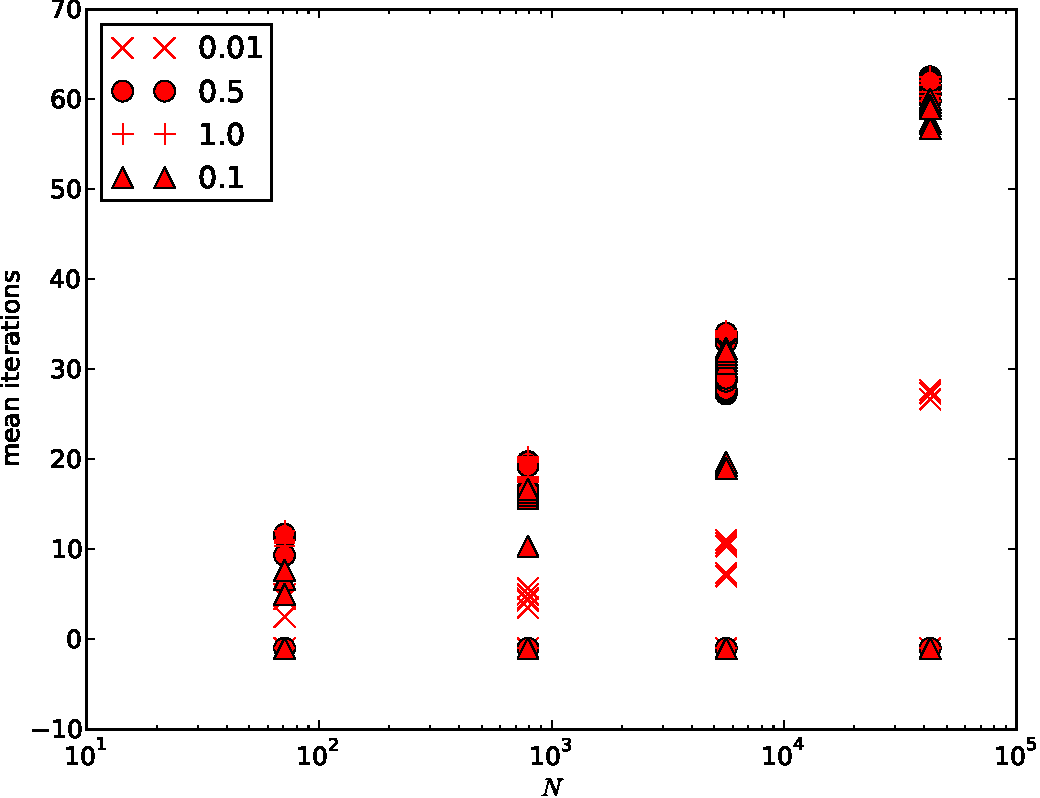
\includegraphics[width=0.8\textwidth]{plots/linear_solvers/ilu-1decoupleddummy-meanofnsolveritersvsinitialnnode.pdf}
  \caption{GMRES iterations to reach relerr $10^{-8}$ for the decoupled LLG preconditioned by ilu-1.}
  \label{fig:its-ilu-decoupled}
\end{figure}

\begin{figure}
  \centering
  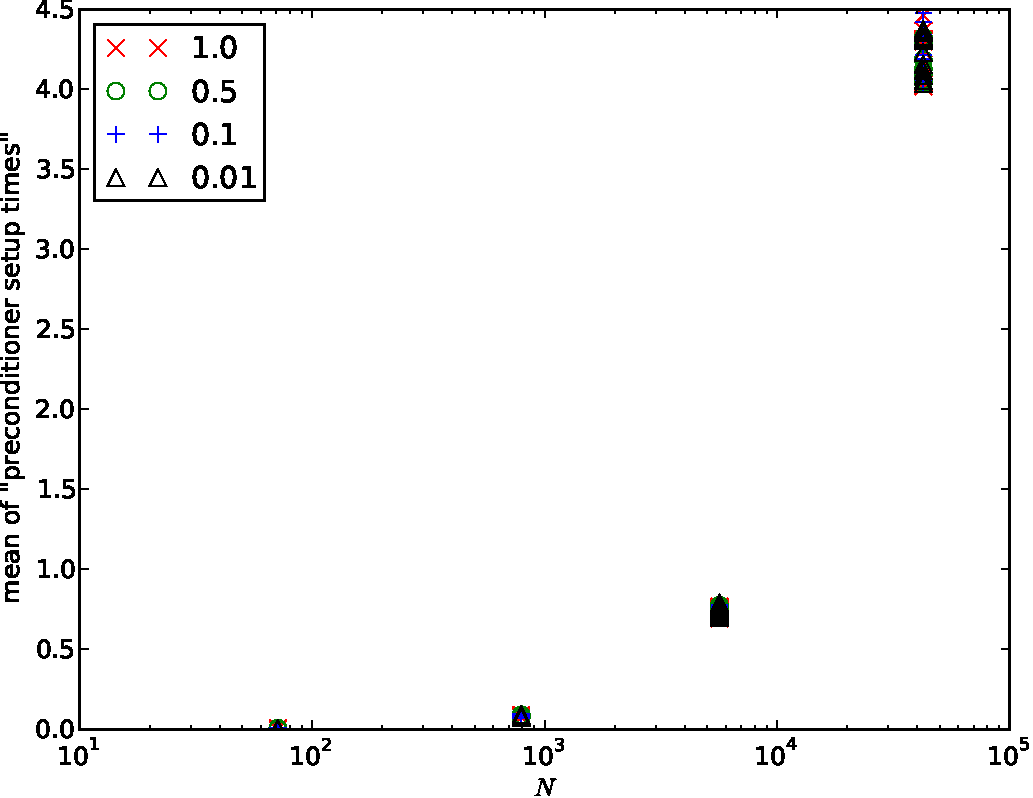
\includegraphics[width=0.8\textwidth]{plots/linear_solvers/ilu-1decoupleddummy-meanofpreconditionersetuptimesvsinitialnnode.pdf}
  \caption{Time to set up an ilu-1 preconditioner for the decoupled LLG block.}
  \label{fig:times-ilu-decoupled}
\end{figure}


Next we consider the preconditioner $\prcd_1$ from \cref{sec:bem-solver-strategies} inverted using a direct solve (LU decomposition).
This is essentially an exact solve without the dense block.
The iteration counts are shown in \cref{fig:its-p1-exact}, they are independent of the number of nodes, time step and all physical parameters.
However the preconditioner setup times, shown in \cref{fig:times-p1-exact} are not so good.
As would be expected from a direct solve they grow rapidly for large systems.

\begin{figure}
  \centering
  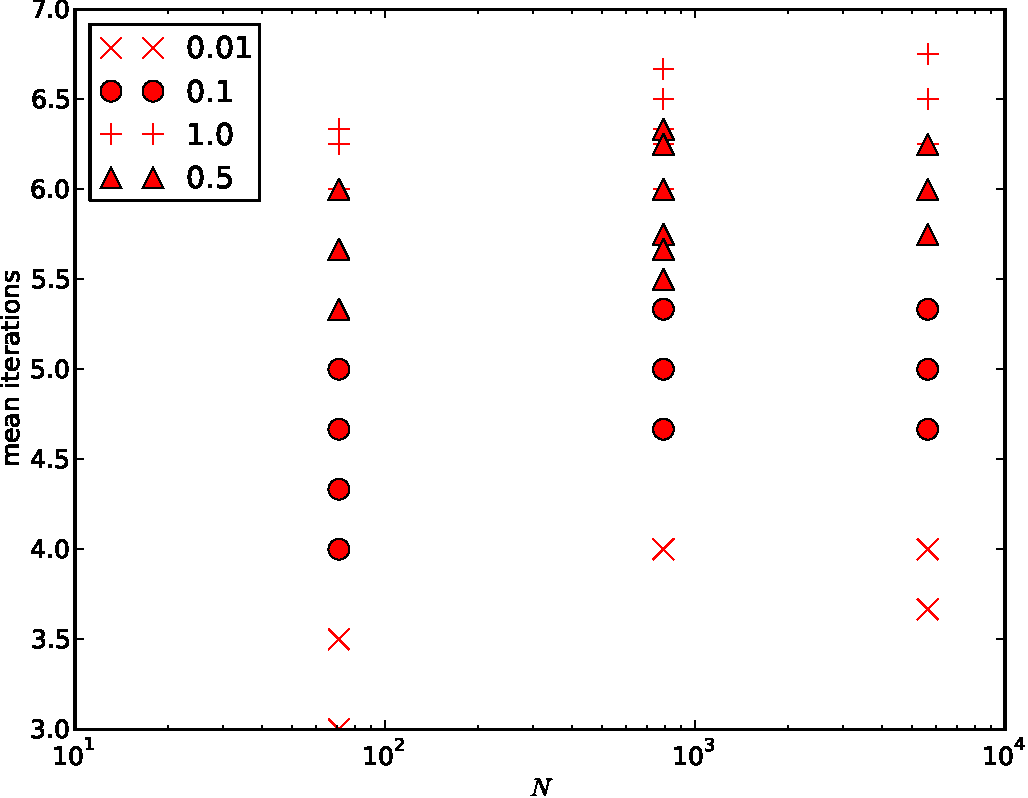
\includegraphics[width=0.8\textwidth]{plots/linear_solvers/som-main-exactimplicitdummy-meanofnsolveritersvsinitialnnode.pdf}
  \caption{Iterations for the monolithic system solved with $\prcd_1$ inverted by LU decomposition.}
  \label{fig:its-p1-exact}
\end{figure}


\begin{figure}
  \centering
  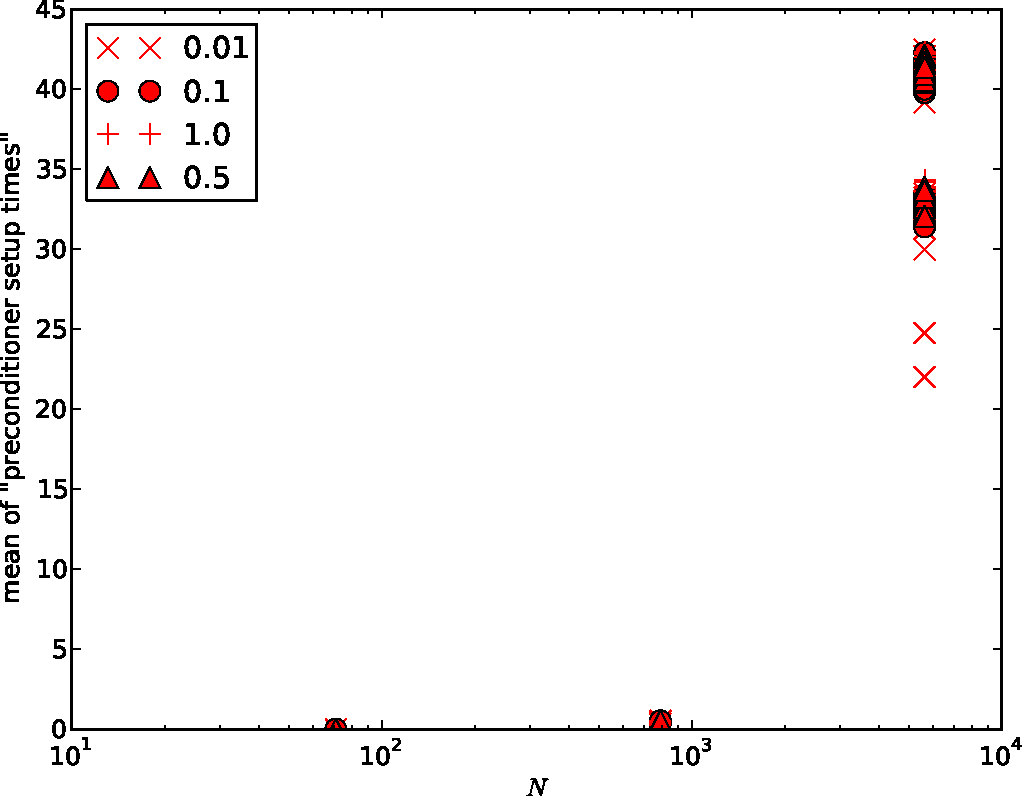
\includegraphics[width=0.8\textwidth]{plots/linear_solvers/som-main-exactimplicitdummy-meanofpreconditionersetuptimesvsinitialnnode.pdf}
  \caption{Preconditioner setup times for $\prcd_1$ inverted by LU decomposition.}
  \label{fig:times-p1-exact}
\end{figure}

The preconditioners $\prcd_2$ and $\prcd_3$ were designed to reduce the setup time.
First we show results for these preconditioners with an exact solve for the $\Fm$ block (and AMG preconditioning, as discussed in \cref{??ds} for the Poisson blocks $\Am$).
The iteration counts are shown in \cref{fig:its-p23-exact}, as with $\prcd_1$ we see that the number of iterations is flat over increasing numbers of nodes, time step size and physical parameters.
The preconditioner setup times are shown in \cref{fig:times-p23-exact}, they are smaller than those in \cref{fig:times-p1-exact} but still grow unacceptably large due to the direct solve of the $\Fm$ block. 

\begin{figure}
  \centering
  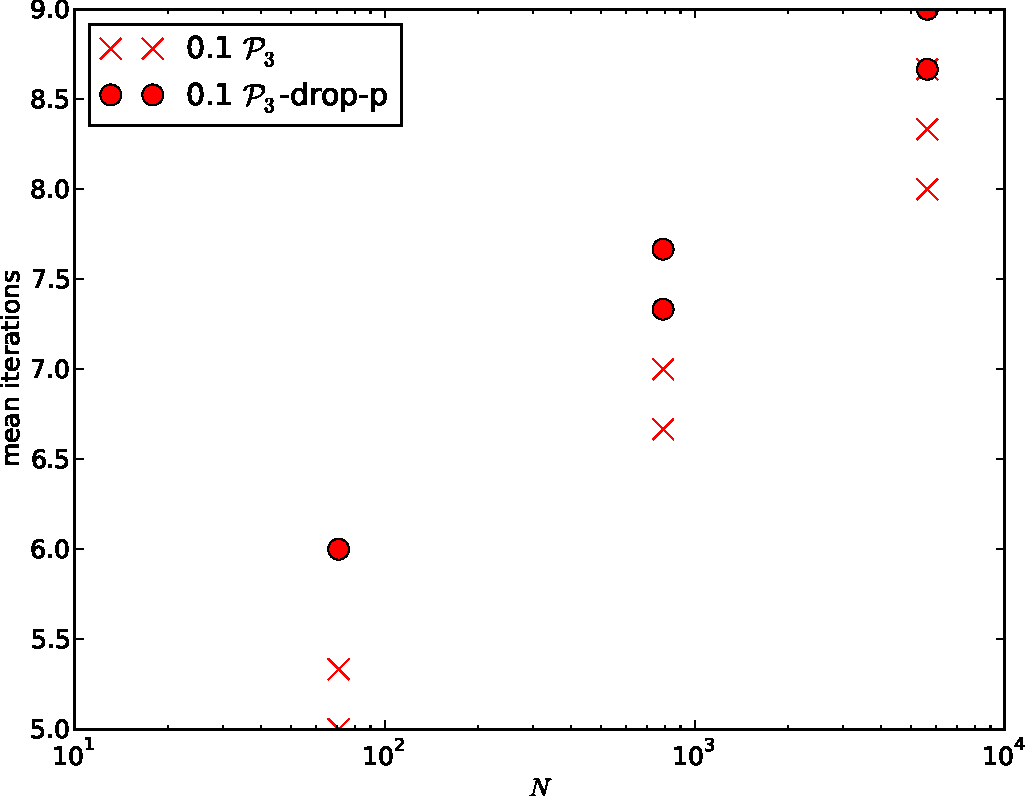
\includegraphics[width=0.8\textwidth]{plots/linear_solvers_p2p3/implicitexact-meanofnsolveritersvsinitialnnode.pdf}
  \caption{Iterations for the monolithic system with $\dtn=0.1$ solved with $\prcd_2$ and $\prcd_3$ with $\Fm$ block inverted by LU decomposition and $\Am$ blocks approximated using AMG.}
  \label{fig:its-p23-exact}
\end{figure}

\begin{figure}
  \centering
  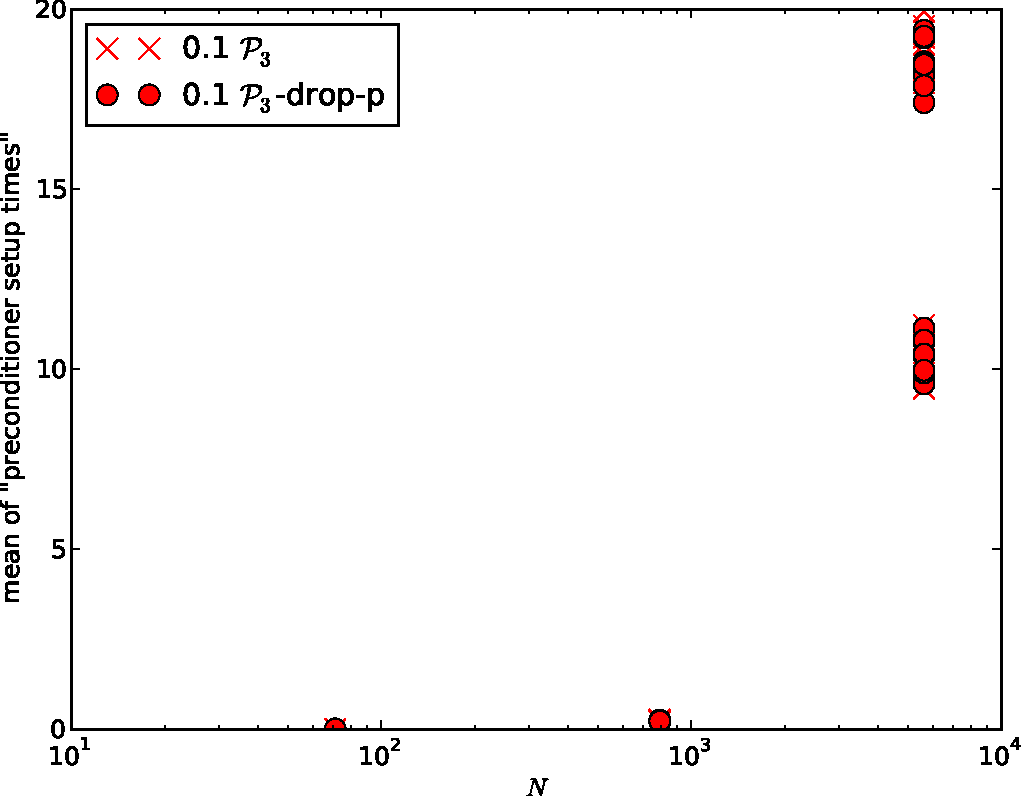
\includegraphics[width=0.8\textwidth]{plots/linear_solvers_p2p3/implicitexact-meanofpreconditionersetuptimesvsinitialnnode.pdf}
  \caption{Preconditioner setup times with $\dtn=0.1$ for $\prcd_2$ and $\prcd_3$ with $\Fm$ block inverted by LU decomposition and $\Am$ blocks approximated using AMG.}
  \label{fig:times-p23-exact}
\end{figure}


Finally we show iteration counts for preconditioners $\prcd_2$ and $\prcd_3$ with the $\Fm$ block solved using the ilu-1 preconditioner.
We cannot expect mesh independent results here, since even the simpler case of the $\Fm$ block alone does not display such behaviour.
The iteration counts shown in \cref{fig:its-p23-ilu1}, are as expected: good at first but ineffective for large meshes.
However the preconditioner set up times, as shown in \cref{fig:times-p23-ilu1} are much better than when using the LU decomposition of the $\Fm$ block. 

\begin{figure}
  \centering
  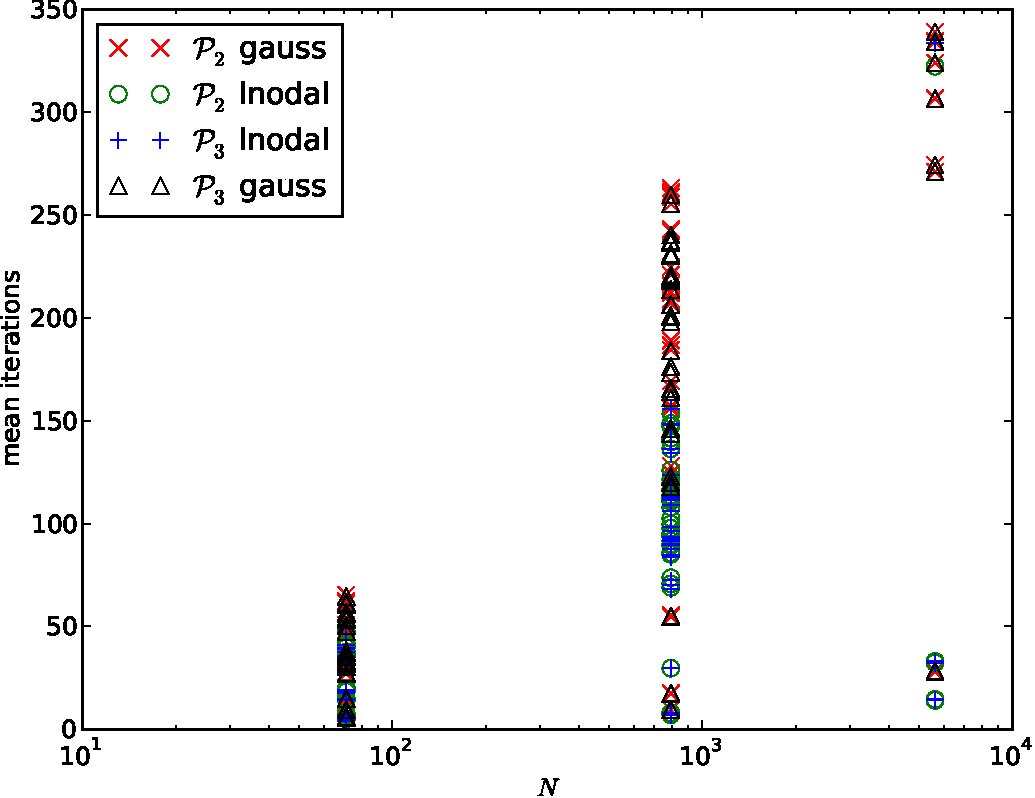
\includegraphics[width=0.8\textwidth]{plots/linear_solvers_p2p3/implicitilu-1-meanofnsolveritersvsinitialnnode.pdf}
  \caption{Iterations for the monolithic system with $\dtn=0.1$ solved with $\prcd_2$ and $\prcd_3$ with $\Fm$ block approximated by ilu-1 and $\Am$ blocks approximated using AMG.}
  \label{fig:its-p23-ilu1}
\end{figure}

\begin{figure}
  \centering
  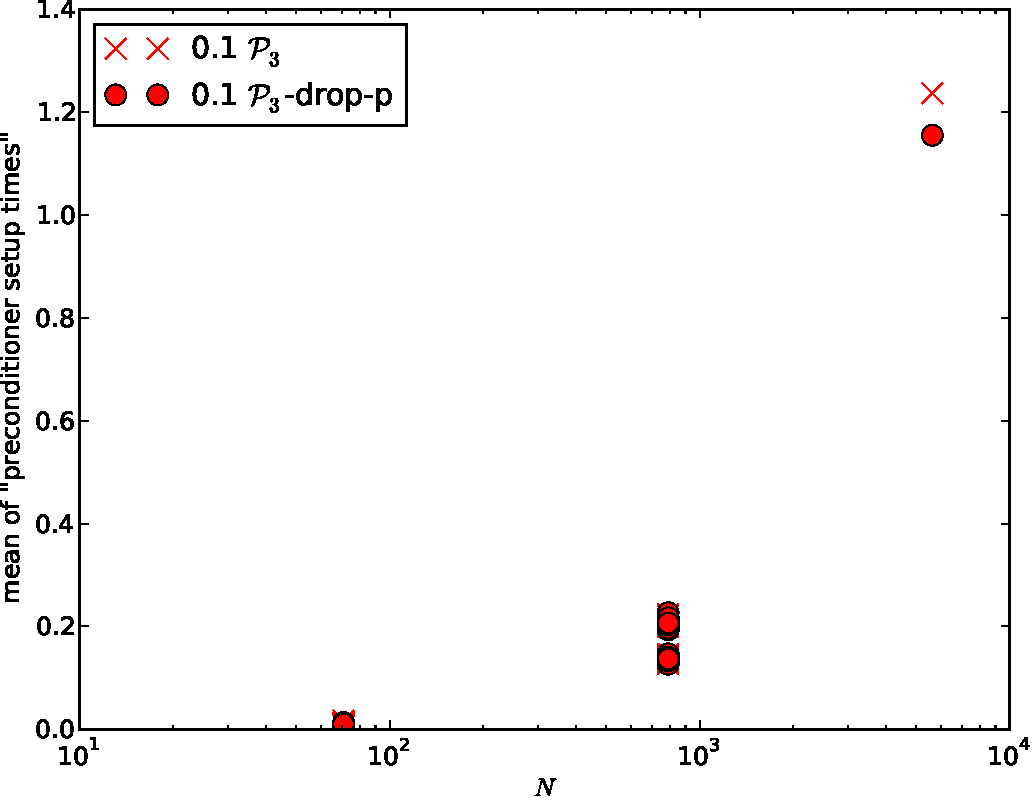
\includegraphics[width=0.8\textwidth]{plots/linear_solvers_p2p3/implicitilu-1-meanofpreconditionersetuptimesvsinitialnnode.pdf}
  \caption{Preconditioner setup times with $\dtn=0.1$ for $\prcd_2$ and $\prcd_3$ with $\Fm$ block approximated by ilu-1 and $\Am$ blocks approximated using AMG.}
  \label{fig:times-p23-ilu1}
\end{figure}

Effect of HLib?

Compare the total solve time for the semi-implicit method (with GMRES and ilu-1 preconditioning) and fully implicit method (with $\prcd_2$, ilu-1 for the $\Fm$ block), both using HLib.
Results are shown in \cref{fig:times-semi-vs-fully-implicit}.
??ds fully implicit a bit slower but not horrible..
Note that in our current implementation the Jacobian assembly time for the fully implicit method is longer than that of the semi-implicit one, however this does not need to be the case with some simple optimisations discussed in \cref{sec:furth-optim-opport}.

\begin{figure}
  \centering
  
\includegraphics[width=0.8\textwidth]{images/placeholder}
  \caption{}
  \label{fig:times-semi-vs-fully-implicit}
\end{figure}


Jacobian assembly times?

Complete solve times?

Poisson? probably no need - known to work extremely well



\section{Outlook}
\label{sec:furth-optim-opport}

In this \thisref{sec:furth-optim-opport} we compare the expected performance of the fully implicit and decoupled approaches with the assumption that a ``sufficiently good'' preconditioner for the $\Fm$ block can be found and discuss further improvements that could be made.

In the fully implicit method timing results presented here the entire FEM Jacobian was recalculated at each Newton step.
This is not actually necessary: the Poisson blocks, $\Am$, and LLG-Poisson coupling blocks, $\Qm$ and $\Pm$, (of \cref{eq:16}) are only dependent on the geometry (\ie the corresponding equations are linear).
Hence these blocks could be precomputed and stored.
This reduces the Jacobian assembly process for the fully implicit method to exactly as the decoupled method.

Similarly the mass matrix sub-blocks on the diagonal of the LLG-block ($\Mm$ of \cref{eq:llg-jacobian}) are only dependent on the geometry.
As an additional optimisation the skew symmetric structure of \cref{eq:llg-jacobian} could be exploited so that the calculation of $\Km_x$ is reused for $-\Km_x$, and similarly for $\Km_y$ and $\Km_z$.
Applying these additional optimisations will reduce the Jacobian calculations to the assembly of three $N \times N$ Jacobian blocks and the magnetocrystalline anisotropy block (which will typically be either $N \times N$ or empty).


Newton residual assembly time is extremely small compared to solve + Jacobian assembly times, so it will be ignored.

So the solve time difference is all that is left: both using Krylov solvers, but fully coupled has extra non-zeros (P, Q, G blocks), approx $4N$ extra elements (base is $11N$), hence approximately half as much time again needed for each Krylov step.
Also fully coupled must use GMRES for all blocks, rather than only for $\Fm$: potentially more expensive orthogonalisation process, could possibly be removed by switching to BiCGStab.
Finally: possible additional iterations, depends on preconditioner used.



\section{Conclusions}

We have demonstrated a fully implicit solver using preconditioned GMRES which is close in terms of cost per linear solve.

For small meshes and/or time steps ILU-1 is a good preconditioner for the LLG block.

Effective mesh independent preconditioners for the $\Fm$ block are badly needed.

AMG and dropping either P or Q is an excellent preconditioner for the Poisson blocks: almost no increase in number of iterations compared to exact!



%%% Local Variables:
%%% mode: latex
%%% TeX-master: "main"
%%% End:
